\providecommand{\Mod}{\mathbb{M}od}
\providecommand{\Fun}{\operatorname{Fun}}
\providecommand{\HomA}{\mathrm{Hom}_{A}}
\providecommand{\HomB}{\mathrm{Hom}_{B}}
\providecommand{\HomC}{\mathrm{Hom}_{C}}
\providecommand{\Homf}{\mathrm{Hom}_{f}}
\providecommand{\Homg}{\mathrm{Hom}_{g}}

\subsection*{练习}

\begin{exercise}\label{ex:restriction-hom-along-functors}
设有\trFunctor{}图表
$E\xrightarrow{k}C\xrightarrow{g}A\xleftarrow{f}B\xleftarrow{h}D$，试计算模
$C\xrightarrow{\HomA(f,g)}B$ 沿\trFunctor{} $k$ 与 $h$ 作限制的结果。
\end{exercise}

\begin{exercise}\label{ex:unital-rings-bimodules-equipment}
证明：幺环、环同态、双模与双模映射也定义一个\trVirtualEquipment。
\end{exercise}

\begin{exercise}\label{ex:two-sided-isofibrations-virtual-equipment}
证明：双侧等价纤维化的\trVirtualDoubleCategory{}连同注 8.1.13 的单位%
\trCell{}一起构成一个\trVirtualEquipment。
\end{exercise}

\section{模的复合}\label{sec:composition-of-modules}

在一个\trVirtualEquipment{}中，并不假定任意一对水平箭头
$A\xrightarrow{E}B$ 与 $B\xrightarrow{F}C$ 都容许一个复合，但存在一套机制，
当某个特定的水平复合 $A\xrightarrow{G}C$ 恰好存在时能将其识别出来。当 $G$ 是
$E$ 与 $F$ 的水平复合时，我们记 $E\otimes F\simeq G$ 或
$\mu\colon E\otimes F\simeq G$，以强化双模类比所提供的直觉。

在模的\trVirtualEquipment{}中，对于模的「水平复合」我们可以赋予两种可能的含
义。第一种含义下，一个复合关系 $\mu\colon E\otimes F\simeq G$ 由一支纤维化
模映射 $\mu\colon E\times_{B}F\xrightarrow{}G$ 见证，后者以与命题 8.2.4 所述%
\trUniversalProperty{}相类比的方式定义一个\trCocartesian\trCell{}（见%
\cref{def:composite}）。这一复合定义可以在任何\trVirtualDoubleCategory{}中给
出，并且在任何\trVirtualEquipment{}——例如模的\trVirtualEquipment——中都表
现良好。可复合模的 $n$ 元序列的复合可以类似地定义。

在模的\trVirtualEquipment{}中，我们形式地定义的所有复合都满足一个更强的、在%
\trInfinityCosmos{}层面表述的\trUniversalProperty。回忆：模
$A\xrightarrow{E}B$、$B\xrightarrow{F}C$ 与 $A\xrightarrow{G}C$ 之间的一支纤
维化映射 $\mu\colon E\times_{B}F\xrightarrow{}G$ 对应于 $A\times C$ 之上的一个%
\trSpan{}映射 $\ulcorner\mu\urcorner\colon E\times_{B}F\to G$ 的纤维化同构
类。说 $\mu$ 在\cref{def:strong-composite}中见证一个\emph{强复合}（strong
composite），其部分含义是要求：它的表示函子对每个模 $A\xrightarrow{H}C$ 都诱
导 Kan 复形的如下\trEquivalence
$-\circ\ulcorner\mu\urcorner\colon\Fun_{A\times C}(G,H)\sim\Fun_{A\times C}(E\times_{B}F,H)$。一旦如此，模 $G$

便可理解为双侧等价纤维化 $E\times_{B}F$ 向诸模之子范畴中的「反射」；然而请注
意，$G$ 与 $E\times_{B}F$ 在 $A\times C$ 之上未必\trEquivalence。定理 7.3.2
的一个特例——它将以\cref{prop:composite-of-legs}的面貌再次出现——就是强复合
的一个实例。

正如这一术语所暗示的，强复合必为复合。既然「作为复合」这一较弱的%
\trUniversalProperty{}在纤维化\trEquivalence{}的意义下刻画了复合模，那么当我
们身处一个保证强复合存在的\trInfinityCosmos{}中时，我们现在引入的 2-范畴式%
\trUniversalProperty{}便足以把它们检测出来。\footnote{这类似于命题 5.2.11 中
所考虑的「定义弱 $p$-笛卡尔变换的\trUniversalProperty{}」与「定义 $p$-笛卡尔
变换的\trUniversalProperty{}」二者之间的关系。}

\begin{definition}\label{def:composite}
模的一个相容序列
\begin{equation*}
A\xrightarrow{E_{1}}A_{1},\ A_{1}\xrightarrow{E_{2}}A_{2},\ \ldots,\
A_{n-1}\xrightarrow{E_{n}}B
\end{equation*}
容许一个\textbf{复合}（composite），如果存在一个模 $A\xrightarrow{E}B$ 与一
个\trCocartesian\trCell
\begin{equation*}
\mu\colon E_{1}\divideontimes\cdots\divideontimes E_{n}\Rightarrow E
\end{equation*}
它由如下\trUniversalProperty{}刻画：任何形如下图的胞腔
\begin{center}
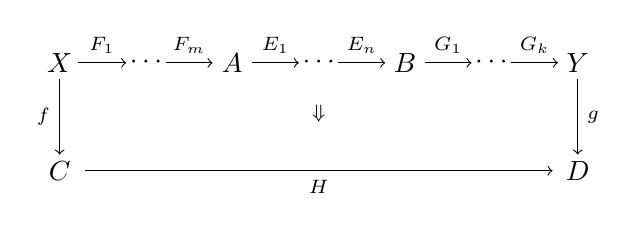
\begin{tikzpicture}[x=1.3em,y=1.3em]
  \node at (0,1.5) {$X$};
  \node at (2.4,1.5) {$\cdots$};
  \node at (4.8,1.5) {$A$};
  \node at (7.2,1.5) {$\cdots$};
  \node at (9.6,1.5) {$B$};
  \node at (12.0,1.5){$\cdots$};
  \node at (14.4,1.5){$Y$};
  \draw[->] (0.5,1.5) -- node[above]{$\scriptstyle F_{1}$} (1.85,1.5);
  \draw[->] (2.95,1.5) -- node[above]{$\scriptstyle F_{m}$} (4.25,1.5);
  \draw[->] (5.35,1.5) -- node[above]{$\scriptstyle E_{1}$} (6.65,1.5);
  \draw[->] (7.75,1.5) -- node[above]{$\scriptstyle E_{n}$} (9.05,1.5);
  \draw[->] (10.15,1.5) -- node[above]{$\scriptstyle G_{1}$} (11.45,1.5);
  \draw[->] (12.55,1.5) -- node[above]{$\scriptstyle G_{k}$} (13.85,1.5);
  \node at (7.2,0.1) {$\scriptstyle\Downarrow$};
  \node at (0,-1.5) {$C$};
  \node at (14.4,-1.5){$D$};
  \draw[->] (0,1.05) -- node[left]{$\scriptstyle f$} (0,-1.05);
  \draw[->] (14.4,1.05) -- node[right]{$\scriptstyle g$} (14.4,-1.05);
  \draw[->] (0.7,-1.5) -- node[below]{$\scriptstyle H$} (13.7,-1.5);
\end{tikzpicture}
\end{center}
都唯一地穿过 $\mu$ 分解，如下所示：
\begin{center}
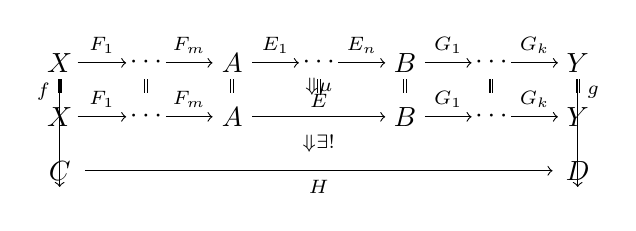
\begin{tikzpicture}[x=1.3em,y=1.3em]
  \node at (0,3.0) {$X$};
  \node at (2.4,3.0) {$\cdots$};
  \node at (4.8,3.0) {$A$};
  \node at (7.2,3.0) {$\cdots$};
  \node at (9.6,3.0) {$B$};
  \node at (12.0,3.0){$\cdots$};
  \node at (14.4,3.0){$Y$};
  \draw[->] (0.5,3.0) -- node[above]{$\scriptstyle F_{1}$} (1.85,3.0);
  \draw[->] (2.95,3.0) -- node[above]{$\scriptstyle F_{m}$} (4.25,3.0);
  \draw[->] (5.35,3.0) -- node[above]{$\scriptstyle E_{1}$} (6.65,3.0);
  \draw[->] (7.75,3.0) -- node[above]{$\scriptstyle E_{n}$} (9.05,3.0);
  \draw[->] (10.15,3.0) -- node[above]{$\scriptstyle G_{1}$} (11.45,3.0);
  \draw[->] (12.55,3.0) -- node[above]{$\scriptstyle G_{k}$} (13.85,3.0);
  \draw[double] (0,2.55) -- (0,2.15);
  \draw[double] (2.4,2.55) -- (2.4,2.15);
  \draw[double] (4.8,2.55) -- (4.8,2.15);
  \draw[double] (7.2,2.55) -- (7.2,2.15);
  \draw[double] (9.6,2.55) -- (9.6,2.15);
  \draw[double] (12.0,2.55) -- (12.0,2.15);
  \draw[double] (14.4,2.55) -- (14.4,2.15);
  \node at (7.2,2.35) {$\scriptstyle\Downarrow\mu$};
  \node at (0,1.5) {$X$};
  \node at (2.4,1.5) {$\cdots$};
  \node at (4.8,1.5) {$A$};
  \node at (9.6,1.5) {$B$};
  \node at (12.0,1.5){$\cdots$};
  \node at (14.4,1.5){$Y$};
  \draw[->] (0.5,1.5) -- node[above]{$\scriptstyle F_{1}$} (1.85,1.5);
  \draw[->] (2.95,1.5) -- node[above]{$\scriptstyle F_{m}$} (4.25,1.5);
  \draw[->] (5.35,1.5) -- node[above]{$\scriptstyle E$} (9.05,1.5);
  \draw[->] (10.15,1.5) -- node[above]{$\scriptstyle G_{1}$} (11.45,1.5);
  \draw[->] (12.55,1.5) -- node[above]{$\scriptstyle G_{k}$} (13.85,1.5);
  \node at (7.2,0.75) {$\scriptstyle\Downarrow\exists!$};
  \node at (0,0) {$C$};
  \node at (14.4,0){$D$};
  \draw[->] (0.7,0) -- node[below]{$\scriptstyle H$} (13.7,0);
  \draw[->] (0,2.55) -- node[left,pos=0.12]{$\scriptstyle f$} (0,-0.45);
  \draw[->] (14.4,2.55) -- node[right,pos=0.12]{$\scriptstyle g$} (14.4,-0.45);
\end{tikzpicture}
\end{center}
\end{definition}

我们已经见过这一定义的一个实例。命题 8.2.4 证明：在模的\trVirtualEquipment{}%
中，诸单位定义零元复合 $\iota\colon\varnothing\Rightarrow \HomA$。

\begin{observation}[复合的唯一性]\label{obs:uniqueness-of-composites}
直接由这一\trUniversalProperty{}可知：在模的\trVirtualEquipment{}中，复合在
竖直\trIsomorphism{}的意义下唯一。回忆引理 8.1.17：平行的诸模在%
\trVirtualEquipment{}中竖直同构，当且仅当它们在通常的纤维化意义下%
\trEquivalence。
\end{observation}

一个复合 $\mu\colon E_{1}\divideontimes\cdots\divideontimes E_{n}\Rightarrow E$ 可以用来缩
减胞腔的定义域：凡出现从 $A$ 到 $B$ 的相容序列
$E_{1}\divideontimes\cdots\divideontimes E_{n}$ 之处，都代之以单个模 $E$。特别是在二元复合
的情形，我们记 $E_{1}\otimes E_{2}$ 表示模 $E_{1}$ 与 $E_{2}$ 的复合——它作
为\trCocartesian\trCell{} $E_{1}\divideontimes E_{2}\Rightarrow E_{1}\otimes E_{2}$
的余定义域出现。请注意，\cref{def:composite}的\trUniversalProperty{}所要求的
多于单纯要求 $\mu\colon E_{1}\divideontimes E_{2}\Rightarrow E_{1}\otimes E_{2}$ 在
源为 $E_{1}\divideontimes E_{2}$ 的诸二元胞腔之中具有普遍性之条件。正如 Hermida 所观察
到的，那较弱的\trUniversalProperty{}不足以证明模的张量积是结合的（见%
\cite{bib53} 的 §8.1 以及\cref{ex:virtual-double-composites}）。相比之下，%
\cref{def:composite}的\trUniversalProperty{}允许我们对三元及更高的复合使用诸
如 $E_{1}\otimes E_{2}\otimes E_{3}$ 的、不带括号的表达式，因为复合在如下意
义上是「结合的」：

\begin{lemma}\label{lem:composite-associativity}
设诸\trCell{} $\mu_{i}\colon E_{i1}\divideontimes\cdots\divideontimes E_{ik_{i}}\Rightarrow E_{i}$（$i=1,\ldots,n$）展示复合。

\begin{enumerate}[label=(\roman*)]
\item 若 $\mu\colon E_{1}\divideontimes\cdots\divideontimes E_{n}\Rightarrow E$ 展示一个复
合，则复合\trCell
\begin{equation*}
E_{11}\divideontimes\cdots\divideontimes E_{nk_{n}}
\xrightarrow{\ \mu_{1}\times\cdots\times\mu_{n}\ }
E_{1}\divideontimes\cdots\divideontimes E_{n}
\xrightarrow{\ \mu\ }
E
\end{equation*}
将 $E$ 展示为序列 $E_{11}\divideontimes\cdots\divideontimes E_{nk_{n}}$ 的一个复合。
\item 若该复合\trCell
\begin{equation*}
E_{11}\divideontimes\cdots\divideontimes E_{nk_{n}}
\xrightarrow{\ \mu_{1}\times\cdots\times\mu_{n}\ }
E_{1}\divideontimes\cdots\divideontimes E_{n}
\xrightarrow{\ \mu\ }
E
\end{equation*}
将 $E$ 展示为序列 $E_{11}\divideontimes\cdots\divideontimes E_{nk_{n}}$ 的一个复合，则
$\mu\colon E_{1}\divideontimes\cdots\divideontimes E_{n}\Rightarrow E$ 将 $E$ 展示为序列
$E_{1}\divideontimes\cdots\divideontimes E_{n}$ 的一个复合。
\end{enumerate}
\end{lemma}

\begin{proof}
对 (i)：所需的双射分解为由映射 $\mu_{1},\ldots,\mu_{n}$ 与 $\mu$ 诱导的
$n+1$ 个双射的复合。对 (ii)：由 $\mu$ 诱导的所需双射与由映射
$\mu_{1},\ldots,\mu_{n}$ 所提供的诸双射复合成一个双射，从而其本身也是一个双
射。
\end{proof}

\begin{remark}\label{rem:fibered-cells-suffice}
由于命题 8.2.1 所确立的限制之\trUniversalProperty，要证明一个\trCell{}
$\mu\colon E_{1}\divideontimes\cdots\divideontimes E_{n}\Rightarrow E$ 在某个%
\trVirtualEquipment{}中展示复合，只需在诸竖直\trFunctor{}皆为恒同的情形——
即所有\trCell{}皆为「\trFibered」之时——证明\cref{def:composite}的分解性质。
\end{remark}

\begin{definition}\label{def:strong-composite}
模的一个相容序列
\begin{equation*}
A\xrightarrow{E_{1}}A_{1},\ A_{1}\xrightarrow{E_{2}}A_{2},\ \ldots,\
A_{n-1}\xrightarrow{E_{n}}B
\end{equation*}
容许一个\textbf{强复合}，如果存在一个模 $A\xrightarrow{E}B$ 与一个%
\trFibered\trCell{} $\mu\colon E_{1}\divideontimes\cdots\divideontimes E_{n}\Rightarrow E$，
它由 $A\times B$ 之上的一个\trFunctor{}
$\ulcorner\mu\urcorner\colon E_{1}\divideontimes\cdots\divideontimes E_{n}\to E$ 表示，使
得对从 $X$ 到 $A$ 的所有相容模序列 $F_{1},\ldots,F_{m}$、从 $B$ 到 $Y$ 的所
有相容模序列 $G_{1},\ldots,G_{k}$ 以及所有模 $X\xrightarrow{H}Y$，这一%
\trFunctor{}都诱导 Kan 复形的如下\trEquivalence
\begin{equation*}
\Fun_{X\times Y}(\vec{F}\times_{A}E\times_{B}\vec{G},\,H)
\xrightarrow[\ \simeq\ ]{\,-\circ(\vec{F}\times_{A}\mu\times_{B}\vec{G})\,}
\Fun_{X\times Y}(\vec{F}\times_{A}E_{1}\times_{A_{1}}\cdots\times_{A_{n-1}}E_{n}\times_{B}\vec{G},\,H)
\end{equation*}
\end{definition}

\begin{lemma}[强复合皆为复合]\label{lem:strong-composites-are-composites}
若 $\mu\colon E_{1}\divideontimes\cdots\divideontimes E_{n}\Rightarrow E$ 是一个强复合，则
$\mu$ 将 $E$ 展示为复合 $E_{1}\otimes\cdots\otimes E_{n}$。
\end{lemma}

\begin{proof}
给定从 $X$ 到 $A$ 的一个相容模序列 $F_{1},\ldots,F_{m}$ 与从 $B$ 到 $Y$ 的
一个相容模序列 $G_{1},\ldots,G_{k}$，作出复合而成的双侧纤维化
$X\overset{q}{\twoheadleftarrow}\vec{F}\overset{p}{\twoheadrightarrow}A$ 与
$B\overset{s}{\twoheadleftarrow}\vec{G}\overset{r}{\twoheadrightarrow}Y$。由%
\cref{rem:fibered-cells-suffice}，只需对余定义域为模 $X\xrightarrow{H}Y$ 的那
些\trFibered{}映射检验复合\trCell{}的\trUniversalProperty。「$\mu$ 是强复合」
这一假设提供了 Kan 复形的\trEquivalence\footnote{原书此显示式右端
$\Fun$ 之下标印作 $A\times B$。按\cref{def:strong-composite}（其中两处下标
均为 $X\times Y$）及此处变元的边界（$H$ 为从 $X$ 到 $Y$ 的模），该下标应为
$X\times Y$，疑原书笔误，此处径改。——译者注}
\begin{equation*}
\Fun_{X\times Y}(\vec{F}\times_{A}E\times_{B}\vec{G},\,H)
\xrightarrow[\ \simeq\ ]{\,-\circ(\vec{F}\times_{A}\mu\times_{B}\vec{G})\,}
\Fun_{X\times Y}(\vec{F}\times_{A}E_{1}\times_{A_{1}}\cdots\times_{A_{n-1}}E_{n}\times_{B}\vec{G},\,H)
\end{equation*}
Kan 复形之间的一个\trEquivalence{}在道路连通分支上定义一个双射，而由观察
8.1.2，每个道路连通分支恰对应于诸\trFunctor{}的一个\trIsomorphism{}类。
\end{proof}

乍看之下，「强复合」的定义显得强得不合理。诸例将产生于命题 8.2.4 之证明所用
的同一结构，该证明展示了在模的\trVirtualEquipment{}中诸单位定义零元复合。

\begin{lemma}\label{lem:fibered-adjoint-strong-composite}
考虑模的\trVirtualEquipment{}中一个 $n$ 元模映射
$\mu\colon E_{1}\divideontimes\cdots\divideontimes E_{n}\Rightarrow E$，其余定义域为从 $A$
到 $B$ 的一个模。若任意一个表示它的\trSpan{}映射
\begin{center}
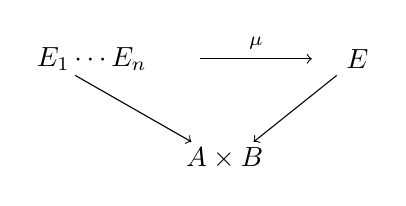
\begin{tikzpicture}[x=1.5em,y=1.5em]
  \node at (0,1.3) {$E_{1}\divideontimes\cdots\divideontimes E_{n}$};
  \node at (6.4,1.3) {$E$};
  \node at (3.2,-1.1) {$A\times B$};
  \draw[->] (2.6,1.3) -- node[above]{$\scriptstyle\ulcorner\mu\urcorner$} (5.3,1.3);
  \draw[->] (-0.4,0.9) -- (2.4,-0.7);
  \draw[->] (5.9,0.9) -- (3.9,-0.7);
\end{tikzpicture}
\end{center}
在 $A\times B$ 之上容许一个\trFiberedAdjunction，则 $\mu$ 将 $E$ 展示为强复合
$E_{1}\otimes\cdots\otimes E_{n}$。
\end{lemma}

\begin{proof}
为检验\cref{def:strong-composite}的\trUniversalProperty，考虑从 $X$ 到 $A$
的一个相容模序列 $F_{1},\ldots,F_{m}$ 与从 $B$ 到 $Y$ 的一个相容模序列
$G_{1},\ldots,G_{k}$，并作出水平复合而成的双侧纤维化
$X\overset{q}{\twoheadleftarrow}\vec{F}\overset{p}{\twoheadrightarrow}A$ 与
$B\overset{s}{\twoheadleftarrow}\vec{G}\overset{r}{\twoheadrightarrow}Y$。所
述的\trFiberedAdjunction{}沿 $p\times s\colon F\times G\to A\times B$ 拉回、沿
$q\times r\colon F\times G\to X\times Y$ 前推，得出一个\trFiberedAdjunction
\begin{center}
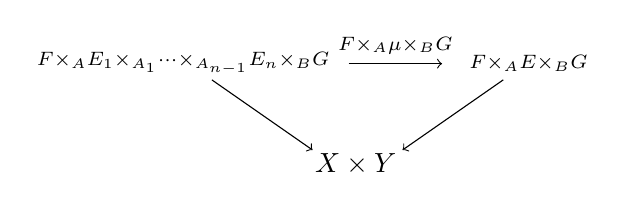
\begin{tikzpicture}[x=1.3em,y=1.3em]
  \node at (0,1.6)
    {$\scriptstyle F\times_{A}E_{1}\times_{A_{1}}\cdots\times_{A_{n-1}}E_{n}\times_{B}G$};
  \node at (9.6,1.6) {$\scriptstyle F\times_{A}E\times_{B}G$};
  \node at (4.8,-1.2) {$X\times Y$};
  \draw[->] (4.6,1.6) -- node[above]{$\scriptstyle F\times_{A}\ulcorner\mu\urcorner\times_{B}G$} (7.2,1.6);
  \draw[->] (0.8,1.15) -- (3.6,-0.8);
  \draw[->] (8.9,1.15) -- (6.1,-0.8);
\end{tikzpicture}
\end{center}
经由\cref{rem:fibered-cells-suffice}，只需对模 $X\xrightarrow{H}Y$ 检验复合
的\trUniversalProperty。由于模是\trDiscrete，施用 $\Fun_{X\times Y}(-,H)$
便将这一\trFiberedAdjunction{}变换为一个\trAdjointEquivalence
\begin{equation*}
\Fun_{X\times Y}(\vec{F}\times_{A}E\times_{B}\vec{G},\,H)
\xrightarrow[\ \simeq\ ]{\,-\circ(\vec{F}\times_{A}\ulcorner\mu\urcorner\times_{B}\vec{G})\,}
\Fun_{X\times Y}(\vec{F}\times_{A}E_{1}\times_{A_{1}}\cdots\times_{A_{n-1}}E_{n}\times_{B}\vec{G},\,H),
\end{equation*}
这就确立了刻画强复合的\trUniversalProperty。
\end{proof}

强复合满足一条与\cref{lem:composite-associativity}相类似的结合性质，其证明亦
类似：

\begin{lemma}\label{lem:strong-composite-associativity}
设诸\trCell{} $\mu_{i}\colon E_{i1}\divideontimes\cdots\divideontimes E_{ik_{i}}\Rightarrow E_{i}$（$i=1,\ldots,n$）展示强复合。

\begin{enumerate}[label=(\roman*)]
\item 若 $\mu\colon E_{1}\divideontimes\cdots\divideontimes E_{n}\Rightarrow E$ 展示一个强
复合，则复合\trCell
\begin{equation*}
E_{11}\divideontimes\cdots\divideontimes E_{nk_{n}}
\xrightarrow{\ \mu_{1}\times\cdots\times\mu_{n}\ }
E_{1}\divideontimes\cdots\divideontimes E_{n}
\xrightarrow{\ \mu\ }
E
\end{equation*}
将 $E$ 展示为序列 $E_{11}\divideontimes\cdots\divideontimes E_{nk_{n}}$ 的一个强复合。
\item 若该复合\trCell
\begin{equation*}
E_{11}\divideontimes\cdots\divideontimes E_{nk_{n}}
\xrightarrow{\ \mu_{1}\times\cdots\times\mu_{n}\ }
E_{1}\divideontimes\cdots\divideontimes E_{n}
\xrightarrow{\ \mu\ }
E
\end{equation*}
将 $E$ 展示为序列 $E_{11}\divideontimes\cdots\divideontimes E_{nk_{n}}$ 的一个强复合，则
$\mu\colon E_{1}\divideontimes\cdots\divideontimes E_{n}\Rightarrow E$ 将 $E$ 展示为序列
$E_{1}\divideontimes\cdots\divideontimes E_{n}$ 的一个强复合。
\end{enumerate}
\end{lemma}

\begin{proof}
\cref{ex:strong-composite-associativity}。
\end{proof}

现在我们转向诸例。复合的诸平凡实例易于验证：

\begin{lemma}\label{lem:trivial-composites}
在模的\trVirtualEquipment{}中：
\begin{enumerate}[label=(\roman*)]
\item 命题 8.2.4 的诸单位 $\iota\colon\varnothing\Rightarrow \HomA$ 定义零元
强复合；
\item 一个一元\trCell{} $\mu\colon E\Rightarrow F$ 是一个复合，当且仅当它在
由从 $A$ 到 $B$ 的诸模与纤维化模映射构成的竖直范畴中是一个\trIsomorphism。
此时，$\mu\colon E\Rightarrow F$ 是一个强复合。
\end{enumerate}
\end{lemma}

\begin{proof}
\cref{ex:trivial-composites-proof}。
\end{proof}

一如所愿，诸单位模 $A\xrightarrow{\HomA}A$ 是\cref{def:composite}所引入的复
合概念的单位，意义如下：对任意模 $A\xrightarrow{E}B$，都存在一个强复合关系
$\HomA\otimes E\otimes \HomB\simeq E$。

\begin{lemma}[与单位的复合]\label{lem:composites-with-units}
对任意模 $A\xrightarrow{E}B$，利用单位\trCell{}的\trUniversalProperty{}定义
的唯一\trCell{} $\circ\colon \HomA\divideontimes E\divideontimes \HomB\Rightarrow E$
\begin{center}
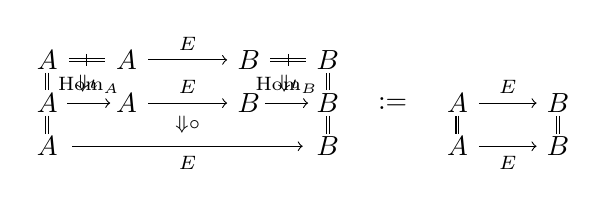
\begin{tikzpicture}[x=1.3em,y=1.3em]
  \node at (0,2.4) {$A$};
  \node at (2.2,2.4) {$A$};
  \node at (5.6,2.4) {$B$};
  \node at (7.8,2.4) {$B$};
  \draw[double] (0.6,2.4) -- (1.6,2.4);\draw (1.1,2.57) -- (1.1,2.23);
  \draw[double] (6.2,2.4) -- (7.2,2.4);\draw (6.7,2.57) -- (6.7,2.23);
  \draw[->] (2.8,2.4) -- node[above]{$\scriptstyle E$} (5.0,2.4);
  \node at (1.1,1.75) {$\scriptstyle\Downarrow\iota$};
  \node at (6.7,1.75) {$\scriptstyle\Downarrow\iota$};
  \node at (0,1.2) {$A$};
  \node at (2.2,1.2) {$A$};
  \node at (5.6,1.2) {$B$};
  \node at (7.8,1.2) {$B$};
  \draw[->] (0.55,1.2) -- node[above]{$\scriptstyle \HomA$} (1.75,1.2);
  \draw[->] (2.8,1.2) -- node[above]{$\scriptstyle E$} (5.0,1.2);
  \draw[->] (6.05,1.2) -- node[above]{$\scriptstyle \HomB$} (7.25,1.2);
  \node at (3.9,0.6) {$\scriptstyle\Downarrow\circ$};
  \node at (0,0) {$A$};
  \node at (7.8,0) {$B$};
  \draw[->] (0.7,0) -- node[below]{$\scriptstyle E$} (7.1,0);
  \draw[double] (0,2.05) -- (0,1.55);
  \draw[double] (0,0.85) -- (0,0.35);
  \draw[double] (7.8,2.05) -- (7.8,1.55);
  \draw[double] (7.8,0.85) -- (7.8,0.35);
  \node at (9.6,1.2) {$:=$};
  \node at (11.4,1.2) {$A$};
  \node at (14.2,1.2) {$B$};
  \draw[->] (12.0,1.2) -- node[above]{$\scriptstyle E$} (13.6,1.2);
  \draw[double] (11.4,0.85) -- (11.4,0.35);
  \draw[double] (14.2,0.85) -- (14.2,0.35);
  \node at (11.4,0) {$A$};
  \node at (14.2,0) {$B$};
  \draw[->] (12.0,0) -- node[below]{$\scriptstyle E$} (13.6,0);
\end{tikzpicture}
\end{center}
将 $E$ 展示为强复合 $\HomA\otimes E\otimes \HomB$。
\end{lemma}

\begin{proof}
本结果由\cref{lem:strong-composite-associativity}(ii) 与%
\cref{lem:trivial-composites}立得。
\end{proof}

\begin{proposition}\label{prop:composite-of-legs}
设 $A\xrightarrow{E}B$ 是由\trSpan{}
$A\overset{q}{\twoheadleftarrow}E\overset{p}{\twoheadrightarrow}B$ 编码的一个
模。那么，由定理 7.1.4(iii) 的\trLeftAdjoint{}与\trRightAdjoint{}之复合所表
示的二元模映射
\begin{center}
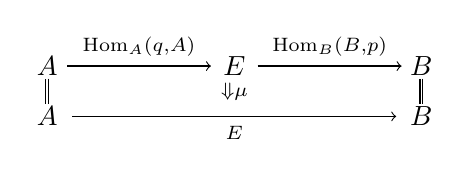
\begin{tikzpicture}[x=1.3em,y=1.3em]
  \node at (0,1.4) {$A$};
  \node at (5.2,1.4) {$E$};
  \node at (10.4,1.4){$B$};
  \draw[->] (0.55,1.4) -- node[above]{$\scriptstyle \HomA(q,A)$} (4.55,1.4);
  \draw[->] (5.85,1.4) -- node[above]{$\scriptstyle \HomB(B,p)$} (9.85,1.4);
  \draw[double] (0,1.05) -- (0,0.35);
  \draw[double] (10.4,1.05) -- (10.4,0.35);
  \node at (5.2,0.7) {$\scriptstyle\Downarrow\mu$};
  \node at (0,0) {$A$};
  \node at (10.4,0){$B$};
  \draw[->] (0.7,0) -- node[below]{$\scriptstyle E$} (9.7,0);
\end{tikzpicture}
\end{center}
展示一个强复合 $\HomA(q,A)\otimes \HomB(B,p)\simeq E$，它把该模表达为代表其
两腿的那些模的复合。
\end{proposition}

\begin{proof}
本结果由定理 7.1.4(iii) 与\cref{lem:fibered-adjoint-strong-composite}（用两
次）立得。\footnote{当然，一个\trLeftAdjoint{}与一个\trRightAdjoint{}的复合
并不是伴随，但这里我们实质上复合的是伴随等价，此时方向无关紧要。}
\end{proof}

\begin{remark}\label{rem:two-sided-fibration-version}
\cref{prop:composite-of-legs}的证明中没有任何一处要求\trSpan{}
$A\overset{q}{\twoheadleftarrow}E\overset{p}{\twoheadrightarrow}B$ 真的是一个
模，而不只是一个单纯的双侧纤维化——唯一的例外是把 $\mu$ 解读为模的%
\trVirtualEquipment{}中的一个二元\trCell。对任意双侧纤维化
$A\overset{q}{\twoheadleftarrow}E\overset{p}{\twoheadrightarrow}B$，沿\trSpan{}%
映射 $\ulcorner\mu\urcorner$ 作限制仍然定义一个双射，其一边是源包含\trSpan{}%
$E$ 且余定义域为模的那些双侧等价纤维化映射，另一边是源转而包含
$\HomA(q,A)\divideontimes \HomB(B,p)$ 的那些映射。特别地，对从 $A$ 到 $B$ 的任意相
容模序列 $E_{1}\divideontimes\cdots\divideontimes E_{n}$，只要其跨度复合定义了双侧纤维化
$A\overset{q}{\twoheadleftarrow}\vec{E}\overset{p}{\twoheadrightarrow}B$，在
模的\trVirtualEquipment{}中的诸模映射之间就存在一个双射\footnote{下右图
中央顶点原书印作 $\vec{E}$。按记号 8.2.7，$\vec{E}$ 表相容序列的复合双侧%
纤维化，而此处顶点应是两支 hom 模 $\HomA(q,A)$ 与 $\HomB(B,p)$ 相会之
对象 $E$，疑原书衍一笔画，此处径改。——译者注}：
\begin{center}
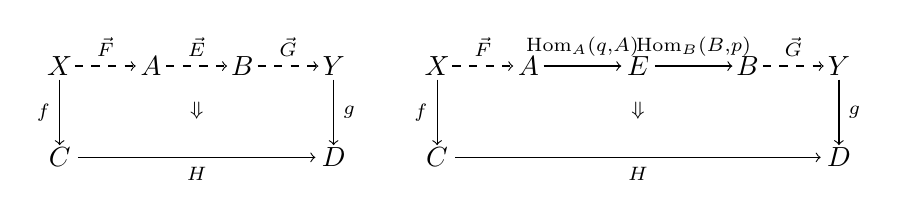
\begin{tikzpicture}[x=1.1em,y=1.1em]
  \node at (0,1.6) {$X$};
  \node at (3.0,1.6) {$A$};
  \node at (6.0,1.6) {$B$};
  \node at (9.0,1.6) {$Y$};
  \draw[->,dashed] (0.5,1.6) -- node[above]{$\scriptstyle\vec{F}$} (2.5,1.6);
  \draw[->,dashed] (3.5,1.6) -- node[above]{$\scriptstyle\vec{E}$} (5.5,1.6);
  \draw[->,dashed] (6.5,1.6) -- node[above]{$\scriptstyle\vec{G}$} (8.5,1.6);
  \node at (4.5,0.15) {$\scriptstyle\Downarrow$};
  \node at (0,-1.4) {$C$};
  \node at (9.0,-1.4){$D$};
  \draw[->] (0,1.15) -- node[left]{$\scriptstyle f$} (0,-1.0);
  \draw[->] (9.0,1.15) -- node[right]{$\scriptstyle g$} (9.0,-1.0);
  \draw[->] (0.6,-1.4) -- node[below]{$\scriptstyle H$} (8.4,-1.4);
  \node at (10.7,0.1) {$\leftrightsquigarrow$};
  \begin{scope}[shift={(12.4,0)}]
  \node at (0,1.6) {$X$};
  \node at (3.0,1.6) {$A$};
  \node at (6.6,1.6) {$E$};
  \node at (10.2,1.6){$B$};
  \node at (13.2,1.6){$Y$};
  \draw[->,dashed] (0.5,1.6) -- node[above]{$\scriptstyle\vec{F}$} (2.5,1.6);
  \draw[->] (3.5,1.6) -- node[above]{$\scriptstyle \HomA(q,A)$} (6.05,1.6);
  \draw[->] (7.15,1.6) -- node[above]{$\scriptstyle \HomB(B,p)$} (9.7,1.6);
  \draw[->,dashed] (10.7,1.6) -- node[above]{$\scriptstyle\vec{G}$} (12.7,1.6);
  \node at (6.6,0.15) {$\scriptstyle\Downarrow$};
  \node at (0,-1.4) {$C$};
  \node at (13.2,-1.4){$D$};
  \draw[->] (0,1.15) -- node[left]{$\scriptstyle f$} (0,-1.0);
  \draw[->] (13.2,1.15) -- node[right]{$\scriptstyle g$} (13.2,-1.0);
  \draw[->] (0.6,-1.4) -- node[below]{$\scriptstyle H$} (12.6,-1.4);
  \end{scope}
\end{tikzpicture}
\end{center}
\end{remark}

\begin{remark}\label{rem:comma-cone-description}
\cref{prop:composite-of-legs}与\cref{rem:two-sided-fibration-version}中的复
合映射 $\mu\colon \HomA(q,A)\divideontimes \HomB(B,p)\Rightarrow E$ 可以用另一种方
式来描述。$\HomA(q,A)$ 与 $\HomB(B,p)$ 的诸\trCommaCone{}定义了一对自然变
换，定理 7.1.4(iv) 的前提适用于它们。
\begin{center}
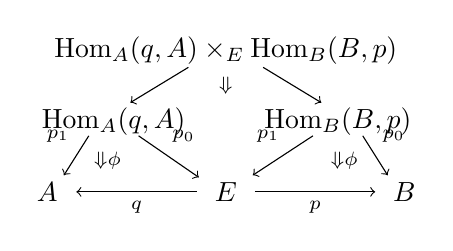
\begin{tikzpicture}[x=1.5em,y=1.5em]
  \node at (0,3.4) {$\HomA(q,A)\times_{E} \HomB(B,p)$};
  \node at (-2.7,1.7) {$\HomA(q,A)$};
  \node at (2.7,1.7) {$\HomB(B,p)$};
  \draw[->] (-0.9,3.0) -- (-2.3,2.15);
  \draw[->] (0.9,3.0) -- (2.3,2.15);
  \node at (0,2.55) {$\scriptstyle\Downarrow$};
  \node at (-4.3,0) {$A$};
  \node at (0,0) {$E$};
  \node at (4.3,0) {$B$};
  \draw[->] (-3.3,1.35) -- node[above left,pos=0.4]{$\scriptstyle p_{1}$} (-3.9,0.4);
  \draw[->] (-2.1,1.35) -- node[above right,pos=0.4]{$\scriptstyle p_{0}$} (-0.65,0.35);
  \node at (-2.85,0.75) {$\scriptstyle\Downarrow\phi$};
  \draw[->] (2.1,1.35) -- node[above left,pos=0.4]{$\scriptstyle p_{1}$} (0.65,0.4);
  \draw[->] (3.3,1.35) -- node[above right,pos=0.4]{$\scriptstyle p_{0}$} (3.9,0.4);
  \node at (2.85,0.75) {$\scriptstyle\Downarrow\phi$};
  \draw[->] (-0.7,0) -- node[below]{$\scriptstyle q$} (-3.6,0);
  \draw[->] (0.7,0) -- node[below]{$\scriptstyle p$} (3.6,0);
\end{tikzpicture}
\end{center}
该结果的结论断言：存在一个良定义的、诸\trFunctor{}的纤维化同构类
$\ulcorner\mu\urcorner\colon \HomA(q,A)\times_{E}\HomB(B,p)\to E$，其定义
是：取左\trCommaCone{}的 $q$-余笛卡尔提升，与右\trCommaCone{}复合，然后取这
一复合\trCell{}的某个 $p$-笛卡尔提升的余定义域——或者先取 $p$-笛卡尔提升，
复合，然后取这一复合的某个 $q$-笛卡尔提升的定义域——此即定理 7.1.4(iii) 记
法下的\trFunctor{} $\ell r\simeq r\ell$。在 $A\xrightarrow{E}B$ 本身是一个逗
号模的情形，所得的诸\trFunctor{}的纤维化同构类 $\ulcorner\mu\urcorner$ 恰是
对如下 2-胞腔进行分类的那一个：该 2-胞腔由所示复合与位于 $E$ 之下的%
\trCommaCone{}粘贴而成。
\end{remark}

任何\trVirtualDoubleCategory{}对每支水平箭头 $A\xrightarrow{E}B$ 都有一个竖直
恒同\trCell，其竖直边界箭头为恒同。在一个\trVirtualEquipment{}中，我们对每支
竖直箭头 $f\colon A\to B$ 还有一个水平一元\textbf{单位\trCell}（unit cell），
其水平边界由命题 8.2.4 的诸单位模 $A\xrightarrow{\HomA}A$ 与
$B\xrightarrow{\HomB}B$ 给出。

\begin{definition}\label{def:unary-unit-cell}
利用 $\Mod(\mathcal{K})$ 中的诸单位模，对任意\trFunctor{} $f\colon A\to B$，
我们可以借助 $A$ 处的零元单位\trCell{}
$\iota\colon\varnothing\Rightarrow \HomA$ 的\trUniversalProperty，通过下右图
的等式来定义如下左图所示的一元单位\trCell：
\begin{center}
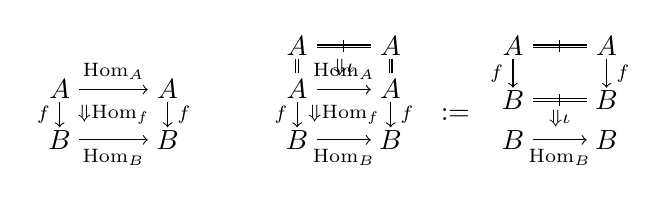
\begin{tikzpicture}[x=1.3em,y=1.3em]
  \node at (0,1.4) {$A$};
  \node at (3.0,1.4) {$A$};
  \draw[->] (0.55,1.4) -- node[above]{$\scriptstyle \HomA$} (2.45,1.4);
  \draw[->] (0,1.05) -- node[left]{$\scriptstyle f$} (0,0.35);
  \draw[->] (3.0,1.05) -- node[right]{$\scriptstyle f$} (3.0,0.35);
  \node at (1.5,0.7) {$\scriptstyle\Downarrow \Homf$};
  \node at (0,0) {$B$};
  \node at (3.0,0) {$B$};
  \draw[->] (0.55,0) -- node[below]{$\scriptstyle \HomB$} (2.45,0);
  \node at (4.7,0.7) {$\leftrightsquigarrow$};
  \begin{scope}[shift={(6.6,0)}]
  \node at (0,2.6) {$A$};
  \node at (2.6,2.6) {$A$};
  \draw[double] (0.55,2.6) -- (2.05,2.6);\draw (1.3,2.77) -- (1.3,2.43);
  \draw[double] (0,2.25) -- (0,1.85);
  \draw[double] (2.6,2.25) -- (2.6,1.85);
  \node at (1.3,2.02) {$\scriptstyle\Downarrow\iota$};
  \node at (0,1.4) {$A$};
  \node at (2.6,1.4) {$A$};
  \draw[->] (0.55,1.4) -- node[above]{$\scriptstyle \HomA$} (2.05,1.4);
  \draw[->] (0,1.05) -- node[left]{$\scriptstyle f$} (0,0.35);
  \draw[->] (2.6,1.05) -- node[right]{$\scriptstyle f$} (2.6,0.35);
  \node at (1.3,0.7) {$\scriptstyle\Downarrow \Homf$};
  \node at (0,0) {$B$};
  \node at (2.6,0) {$B$};
  \draw[->] (0.55,0) -- node[below]{$\scriptstyle \HomB$} (2.05,0);
  \end{scope}
  \node at (11.0,0.7) {$:=$};
  \begin{scope}[shift={(12.6,0)}]
  \node at (0,2.6) {$A$};
  \node at (2.6,2.6) {$A$};
  \draw[double] (0.55,2.6) -- (2.05,2.6);\draw (1.3,2.77) -- (1.3,2.43);
  \draw[->] (0,2.25) -- node[left]{$\scriptstyle f$} (0,1.45);
  \draw[->] (2.6,2.25) -- node[right]{$\scriptstyle f$} (2.6,1.45);
  \node at (0,1.1) {$B$};
  \node at (2.6,1.1) {$B$};
  \draw[double] (0.55,1.1) -- (2.05,1.1);\draw (1.3,1.27) -- (1.3,0.93);
  \node at (1.3,0.58) {$\scriptstyle\Downarrow\iota$};
  \node at (0,0) {$B$};
  \node at (2.6,0) {$B$};
  \draw[->] (0.55,0) -- node[below]{$\scriptstyle \HomB$} (2.05,0);
  \end{scope}
\end{tikzpicture}
\end{center}
\end{definition}

在引理 8.1.16 的刻画中，定义一元单位\trCell{}的粘贴等式的两边都对应于如下所
示的恒同 2-胞腔：
\begin{center}
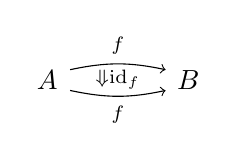
\begin{tikzpicture}[x=1.5em,y=1.5em]
  \node at (0,0.9) {$A$};
  \node at (3.4,0.9) {$B$};
  \draw[->] (0.55,1.15) to[bend left=12] node[above]{$\scriptstyle f$} (2.85,1.15);
  \draw[->] (0.55,0.65) to[bend right=12] node[below]{$\scriptstyle f$} (2.85,0.65);
  \node at (1.7,0.9) {$\scriptstyle\Downarrow\mathrm{id}_{f}$};
\end{tikzpicture}
\end{center}

一如所愿，在模的\trVirtualEquipment{}中，诸单位\trCell{}是诸\trCell{}的竖直
复合的单位。

\begin{lemma}[与单位\trCell{}的复合]\label{lem:composition-with-unit-cells}
任何如下右图所示的\trCell{} $\alpha$ 都等于如下左图所示的粘贴复合\footnote{%
原书引理 8.3.15 的两对粘贴图（本图与证明图，p.328--329）的四条 $B\to C$ 底边均
印作 $\vec{E}$。按记号 8.2.7，$\vec{E}$ 专指序列
$E_{1}\divideontimes\cdots\divideontimes E_{n}$（$A_{0}\to A_{n}$ 方向）的复合
双侧纤维化，标于 $B\to C$ 之边无义；且外侧胞腔之靶即 $\circ$ 之靶（由引理
8.3.10，$\circ$ 之靶为模 $E\colon B\to C$），恒同胞腔之分解亦要求上下边相%
一致。四处径改。——译者注}：
\begin{center}
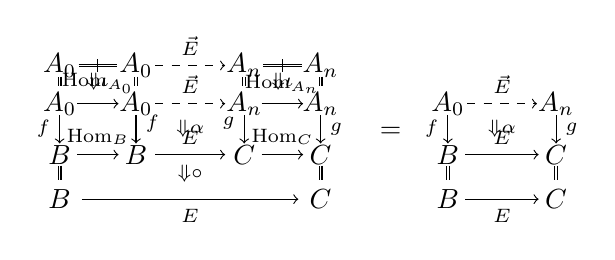
\begin{tikzpicture}[x=1.15em,y=1.15em]
  \node at (0,3.6) {$A_{0}$};
  \node at (2.4,3.6) {$A_{0}$};
  \node at (5.8,3.6) {$A_{n}$};
  \node at (8.2,3.6) {$A_{n}$};
  \draw[double] (0.6,3.6) -- (1.8,3.6);\draw (1.2,3.79) -- (1.2,3.41);
  \draw[double] (6.4,3.6) -- (7.6,3.6);\draw (7.0,3.79) -- (7.0,3.41);
  \draw[->,dashed] (3.0,3.6) -- node[above]{$\scriptstyle\vec{E}$} (5.2,3.6);
  \draw[double] (0,3.25) -- (0,2.95);
  \draw[double] (2.4,3.25) -- (2.4,2.95);
  \draw[double] (5.8,3.25) -- (5.8,2.95);
  \draw[double] (8.2,3.25) -- (8.2,2.95);
  \node at (1.2,3.1) {$\scriptstyle\Downarrow\iota$};
  \node at (7.0,3.1) {$\scriptstyle\Downarrow\iota$};
  \node at (0,2.4) {$A_{0}$};
  \node at (2.4,2.4) {$A_{0}$};
  \node at (5.8,2.4) {$A_{n}$};
  \node at (8.2,2.4) {$A_{n}$};
  \draw[->] (0.55,2.4) -- node[above]{$\scriptstyle \mathrm{Hom}_{A_{0}}$} (1.85,2.4);
  \draw[->,dashed] (3.0,2.4) -- node[above]{$\scriptstyle\vec{E}$} (5.2,2.4);
  \draw[->] (6.35,2.4) -- node[above]{$\scriptstyle \mathrm{Hom}_{A_{n}}$} (7.65,2.4);
  \draw[->] (0,2.05) -- node[left]{$\scriptstyle f$} (0,1.15);
  \draw[->] (2.4,2.05) -- node[right,pos=0.3]{$\scriptstyle f$} (2.4,1.15);
  \node at (4.1,1.6) {$\scriptstyle\Downarrow\alpha$};
  \draw[->] (5.8,2.05) -- node[left,pos=0.3]{$\scriptstyle g$} (5.8,1.15);
  \draw[->] (8.2,2.05) -- node[right]{$\scriptstyle g$} (8.2,1.15);
  \node at (0,0.8) {$B$};
  \node at (2.4,0.8) {$B$};
  \node at (5.8,0.8) {$C$};
  \node at (8.2,0.8) {$C$};
  \draw[->] (0.55,0.8) -- node[above]{$\scriptstyle \HomB$} (1.85,0.8);
  \draw[->] (3.0,0.8) -- node[above]{$\scriptstyle E$} (5.2,0.8);
  \draw[->] (6.35,0.8) -- node[above]{$\scriptstyle \HomC$} (7.65,0.8);
  \node at (4.1,0.2) {$\scriptstyle\Downarrow\circ$};
  \draw[double] (0,0.45) -- (0,0.0);
  \draw[double] (8.2,0.45) -- (8.2,0.0);
  \node at (0,-0.6) {$B$};
  \node at (8.2,-0.6){$C$};
  \draw[->] (0.7,-0.6) -- node[below]{$\scriptstyle E$} (7.5,-0.6);
  \node at (10.4,1.5) {$=$};
  \begin{scope}[shift={(12.2,0)}]
  \node at (0,2.4) {$A_{0}$};
  \node at (3.4,2.4) {$A_{n}$};
  \draw[->,dashed] (0.6,2.4) -- node[above]{$\scriptstyle\vec{E}$} (2.8,2.4);
  \draw[->] (0,2.05) -- node[left]{$\scriptstyle f$} (0,1.15);
  \draw[->] (3.4,2.05) -- node[right]{$\scriptstyle g$} (3.4,1.15);
  \node at (1.7,1.6) {$\scriptstyle\Downarrow\alpha$};
  \node at (0,0.8) {$B$};
  \node at (3.4,0.8) {$C$};
  \draw[->] (0.55,0.8) -- node[above]{$\scriptstyle E$} (2.85,0.8);
  \draw[double] (0,0.45) -- (0,0.0);
  \draw[double] (3.4,0.45) -- (3.4,0.0);
  \node at (0,-0.6) {$B$};
  \node at (3.4,-0.6){$C$};
  \draw[->] (0.55,-0.6) -- node[below]{$\scriptstyle E$} (2.85,-0.6);
  \end{scope}
\end{tikzpicture}
\end{center}
\end{lemma}

\begin{proof}
由\cref{def:unary-unit-cell}与定义 8.1.8 所陈述的、\trVirtualDoubleCategory{}%
中与恒同\trCell{}复合的诸定律，所述等式的左边复合等于下面展示的左边复合%
\trCell，而所述等式的右边等于下面展示的右边复合\trCell：
\begin{center}
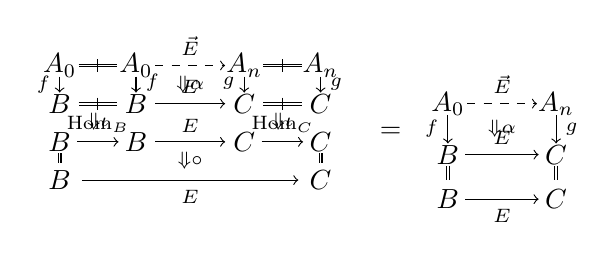
\begin{tikzpicture}[x=1.15em,y=1.15em]
  \node at (0,3.6) {$A_{0}$};
  \node at (2.4,3.6) {$A_{0}$};
  \node at (5.8,3.6) {$A_{n}$};
  \node at (8.2,3.6) {$A_{n}$};
  \draw[double] (0.6,3.6) -- (1.8,3.6);\draw (1.2,3.79) -- (1.2,3.41);
  \draw[double] (6.4,3.6) -- (7.6,3.6);\draw (7.0,3.79) -- (7.0,3.41);
  \draw[->,dashed] (3.0,3.6) -- node[above]{$\scriptstyle\vec{E}$} (5.2,3.6);
  \draw[->] (0,3.25) -- node[left]{$\scriptstyle f$} (0,2.75);
  \draw[->] (2.4,3.25) -- node[right,pos=0.4]{$\scriptstyle f$} (2.4,2.75);
  \node at (4.1,3.0) {$\scriptstyle\Downarrow\alpha$};
  \draw[->] (5.8,3.25) -- node[left,pos=0.4]{$\scriptstyle g$} (5.8,2.75);
  \draw[->] (8.2,3.25) -- node[right]{$\scriptstyle g$} (8.2,2.75);
  \node at (0,2.4) {$B$};
  \node at (2.4,2.4) {$B$};
  \node at (5.8,2.4) {$C$};
  \node at (8.2,2.4) {$C$};
  \draw[double] (0.6,2.4) -- (1.8,2.4);\draw (1.2,2.59) -- (1.2,2.21);
  \draw[->] (3.0,2.4) -- node[above]{$\scriptstyle E$} (5.2,2.4);
  \draw[double] (6.4,2.4) -- (7.6,2.4);\draw (7.0,2.59) -- (7.0,2.21);
  \node at (1.2,1.85) {$\scriptstyle\Downarrow\iota$};
  \node at (7.0,1.85) {$\scriptstyle\Downarrow\iota$};
  \node at (0,1.2) {$B$};
  \node at (2.4,1.2) {$B$};
  \node at (5.8,1.2) {$C$};
  \node at (8.2,1.2) {$C$};
  \draw[->] (0.55,1.2) -- node[above]{$\scriptstyle \HomB$} (1.85,1.2);
  \draw[->] (3.0,1.2) -- node[above]{$\scriptstyle E$} (5.2,1.2);
  \draw[->] (6.35,1.2) -- node[above]{$\scriptstyle \HomC$} (7.65,1.2);
  \node at (4.1,0.6) {$\scriptstyle\Downarrow\circ$};
  \draw[double] (0,0.85) -- (0,0.55);
  \draw[double] (8.2,0.85) -- (8.2,0.55);
  \node at (0,0) {$B$};
  \node at (8.2,0) {$C$};
  \draw[->] (0.7,0) -- node[below]{$\scriptstyle E$} (7.5,0);
  \node at (10.4,1.5) {$=$};
  \begin{scope}[shift={(12.2,0)}]
  \node at (0,2.4) {$A_{0}$};
  \node at (3.4,2.4) {$A_{n}$};
  \draw[->,dashed] (0.6,2.4) -- node[above]{$\scriptstyle\vec{E}$} (2.8,2.4);
  \draw[->] (0,2.05) -- node[left]{$\scriptstyle f$} (0,1.15);
  \draw[->] (3.4,2.05) -- node[right]{$\scriptstyle g$} (3.4,1.15);
  \node at (1.7,1.6) {$\scriptstyle\Downarrow\alpha$};
  \node at (0,0.8) {$B$};
  \node at (3.4,0.8) {$C$};
  \draw[->] (0.55,0.8) -- node[above]{$\scriptstyle E$} (2.85,0.8);
  \draw[double] (0,0.45) -- (0,0.0);
  \draw[double] (3.4,0.45) -- (3.4,0.0);
  \node at (0,-0.6) {$B$};
  \node at (3.4,-0.6){$C$};
  \draw[->] (0.55,-0.6) -- node[below]{$\scriptstyle E$} (2.85,-0.6);
  \end{scope}
\end{tikzpicture}
\end{center}
由\cref{lem:composites-with-units}，左边等于右边。
\end{proof}

\begin{definition}[胞腔的水平复合]\label{def:horizontal-composite-cells}
若给定一个水平相容的一元\trCell{}序列
\begin{center}
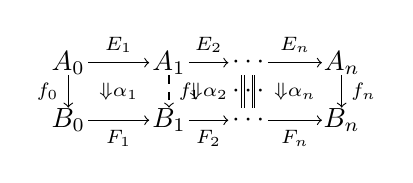
\begin{tikzpicture}[x=1.3em,y=1.3em]
  \node at (0,1.6) {$A_{0}$};
  \node at (2.8,1.6) {$A_{1}$};
  \node at (5.0,1.6) {$\cdots$};
  \node at (7.6,1.6) {$A_{n}$};
  \draw[->] (0.55,1.6) -- node[above]{$\scriptstyle E_{1}$} (2.25,1.6);
  \draw[->] (3.35,1.6) -- node[above]{$\scriptstyle E_{2}$} (4.45,1.6);
  \draw[->] (5.55,1.6) -- node[above]{$\scriptstyle E_{n}$} (7.05,1.6);
  \draw[->] (0,1.25) -- node[left]{$\scriptstyle f_{0}$} (0,0.35);
  \node at (1.4,0.8) {$\scriptstyle\Downarrow\alpha_{1}$};
  \draw[->,dashed] (2.8,1.25) -- node[right]{$\scriptstyle f_{1}$} (2.8,0.35);
  \node at (3.9,0.8) {$\scriptstyle\Downarrow\alpha_{2}$};
  \draw[double] (4.85,1.25) -- (4.85,0.35);
  \draw[double] (5.15,1.25) -- (5.15,0.35);
  \node at (5.0,0.8) {$\cdots$};
  \node at (6.3,0.8) {$\scriptstyle\Downarrow\alpha_{n}$};
  \draw[->] (7.6,1.25) -- node[right]{$\scriptstyle f_{n}$} (7.6,0.35);
  \node at (0,0) {$B_{0}$};
  \node at (2.8,0) {$B_{1}$};
  \node at (5.0,0) {$\cdots$};
  \node at (7.6,0) {$B_{n}$};
  \draw[->] (0.55,0) -- node[below]{$\scriptstyle F_{1}$} (2.25,0);
  \draw[->] (3.35,0) -- node[below]{$\scriptstyle F_{2}$} (4.45,0);
  \draw[->] (5.55,0) -- node[below]{$\scriptstyle F_{n}$} (7.05,0);
\end{tikzpicture}
\end{center}
使得相容序列 $E_{1}\divideontimes\cdots\divideontimes E_{n}$ 与
$F_{1}\divideontimes\cdots\divideontimes F_{n}$ 都容许复合，那么就存在一个\textbf{水平复合
一元\trCell}（horizontal composite unary cell）
$\alpha_{1}*\cdots *\alpha_{n}$，它在给定复合
$\circ\colon E_{1}\divideontimes\cdots\divideontimes E_{n}\Rightarrow E$ 与
$F_{1}\divideontimes\cdots\divideontimes F_{n}\Rightarrow F$ 的取法之下，由如下粘贴等式唯
一确定：
\begin{rveq}\label{eq:horizontal-composite-pasting}
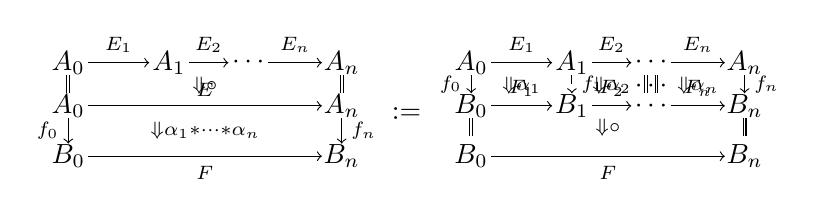
\begin{tikzpicture}[x=1.3em,y=1.3em]
  \node at (0,2.6) {$A_{0}$};
  \node at (2.8,2.6) {$A_{1}$};
  \node at (5.0,2.6) {$\cdots$};
  \node at (7.6,2.6) {$A_{n}$};
  \draw[->] (0.55,2.6) -- node[above]{$\scriptstyle E_{1}$} (2.25,2.6);
  \draw[->] (3.35,2.6) -- node[above]{$\scriptstyle E_{2}$} (4.45,2.6);
  \draw[->] (5.55,2.6) -- node[above]{$\scriptstyle E_{n}$} (7.05,2.6);
  \draw[double] (0,2.25) -- (0,1.75);
  \draw[double] (7.6,2.25) -- (7.6,1.75);
  \node at (3.8,1.95) {$\scriptstyle\Downarrow\circ$};
  \node at (0,1.4) {$A_{0}$};
  \node at (7.6,1.4) {$A_{n}$};
  \draw[->] (0.55,1.4) -- node[above]{$\scriptstyle E$} (7.05,1.4);
  \draw[->] (0,1.05) -- node[left]{$\scriptstyle f_{0}$} (0,0.35);
  \node at (3.8,0.7) {$\scriptstyle\Downarrow\alpha_{1}*\cdots *\alpha_{n}$};
  \draw[->] (7.6,1.05) -- node[right]{$\scriptstyle f_{n}$} (7.6,0.35);
  \node at (0,0) {$B_{0}$};
  \node at (7.6,0) {$B_{n}$};
  \draw[->] (0.55,0) -- node[below]{$\scriptstyle F$} (7.05,0);
  \node at (9.4,1.2) {$:=$};
  \begin{scope}[shift={(11.2,0)}]
  \node at (0,2.6) {$A_{0}$};
  \node at (2.8,2.6) {$A_{1}$};
  \node at (5.0,2.6) {$\cdots$};
  \node at (7.6,2.6) {$A_{n}$};
  \draw[->] (0.55,2.6) -- node[above]{$\scriptstyle E_{1}$} (2.25,2.6);
  \draw[->] (3.35,2.6) -- node[above]{$\scriptstyle E_{2}$} (4.45,2.6);
  \draw[->] (5.55,2.6) -- node[above]{$\scriptstyle E_{n}$} (7.05,2.6);
  \draw[->] (0,2.25) -- node[left]{$\scriptstyle f_{0}$} (0,1.75);
  \node at (1.4,1.95) {$\scriptstyle\Downarrow\alpha_{1}$};
  \draw[->,dashed] (2.8,2.25) -- node[right]{$\scriptstyle f_{1}$} (2.8,1.75);
  \node at (3.9,1.95) {$\scriptstyle\Downarrow\alpha_{2}$};
  \draw[double] (4.85,2.25) -- (4.85,1.75);
  \draw[double] (5.15,2.25) -- (5.15,1.75);
  \node at (5.0,1.95) {$\cdots$};
  \node at (6.3,1.95) {$\scriptstyle\Downarrow\alpha_{n}$};
  \draw[->] (7.6,2.25) -- node[right]{$\scriptstyle f_{n}$} (7.6,1.75);
  \node at (0,1.4) {$B_{0}$};
  \node at (2.8,1.4) {$B_{1}$};
  \node at (5.0,1.4) {$\cdots$};
  \node at (7.6,1.4) {$B_{n}$};
  \draw[->] (0.55,1.4) -- node[above]{$\scriptstyle F_{1}$} (2.25,1.4);
  \draw[->] (3.35,1.4) -- node[above]{$\scriptstyle F_{2}$} (4.45,1.4);
  \draw[->] (5.55,1.4) -- node[above]{$\scriptstyle F_{n}$} (7.05,1.4);
  \draw[double] (0,1.05) -- (0,0.55);
  \draw[double] (7.6,1.05) -- (7.6,0.55);
  \node at (3.8,0.8) {$\scriptstyle\Downarrow\circ$};
  \node at (0,0) {$B_{0}$};
  \node at (7.6,0) {$B_{n}$};
  \draw[->] (0.55,0) -- node[below]{$\scriptstyle F$} (7.05,0);
  \end{scope}
\end{tikzpicture}
\end{rveq}
\end{definition}

通过一个与\cref{lem:composition-with-unit-cells}之证明十分类似的论证（其中
用到\cref{lem:composites-with-units}的诸复合），一元\trCell{} $\alpha$ 与位
于其竖直边界\trFunctor{}处的单位\trCell{} $\Homf$ 与 $\Homg$ 的水平复合
$\Homf*\alpha*\Homg$ 复原了 $\alpha$（见\cref{ex:unit-cells-recover-alpha}）。
利用\cref{def:horizontal-composite-cells}的一元\trCell{}水平复合，我们可以
把 $\Mod(\mathcal{K})$ 理解为包含各种「竖直的」与「水平的」\trBicategory。

\begin{proposition}[虚拟装备中的竖直 2-范畴]\label{prop:vertical-two-category}
任何\trVirtualEquipment{}都包含一个\textbf{竖直 2-范畴}（vertical
2-category）：其对象是该\trVirtualEquipment{}的对象，其箭头是竖直箭头，其
2-胞腔是如下所示的那些一元\trCell——即水平边界箭头由诸单位模给出的那些：
\begin{center}
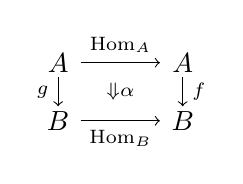
\begin{tikzpicture}[x=1.5em,y=1.5em]
  \node at (0,1.4) {$A$};
  \node at (3.0,1.4) {$A$};
  \draw[->] (0.55,1.4) -- node[above]{$\scriptstyle \HomA$} (2.45,1.4);
  \draw[->] (0,1.05) -- node[left]{$\scriptstyle g$} (0,0.35);
  \draw[->] (3.0,1.05) -- node[right]{$\scriptstyle f$} (3.0,0.35);
  \node at (1.5,0.7) {$\scriptstyle\Downarrow\alpha$};
  \node at (0,0) {$B$};
  \node at (3.0,0) {$B$};
  \draw[->] (0.55,0) -- node[below]{$\scriptstyle \HomB$} (2.45,0);
\end{tikzpicture}
\end{center}
\end{proposition}

\begin{proof}
为证明这些结构定义一个 2-范畴，我们必须——采用定义 B.1.1 的标准术语——定
义 2-胞腔的「水平」复合（沿一个边界 0-\trCell{}复合）与「竖直」复合（沿一个
边界 1-\trCell{}复合）。2-范畴中的「水平」复合经由\trVirtualDoubleCategory{}%
中的竖直复合来定义，后者见定义 8.1.8；2-范畴中的「竖直」复合则由%
\cref{def:horizontal-composite-cells}定义。为看出所得者是 2-范畴而非\trBicategory，请注意：任何 1-胞腔的复合严格结合且严格幺的\trBicategory{}都是 2-范畴；而在此
处，1-胞腔是该\trVirtualDoubleCategory{}的竖直箭头，它们确实严格复合。
\end{proof}

在命题 8.4.11 中我们将证明：\trVirtualEquipment{} $\Mod(\mathcal{K})$ 中的竖
直 2-范畴同构于\trHomotopyTwoCategory{} $\mathfrak{h}\mathcal{K}$。

\begin{remark}[虚拟装备中的水平\trBicategory]\label{rem:horizontal-bicategories}
经由\cref{def:horizontal-composite-cells}，一个\trVirtualEquipment{}也可以被
理解为包含各种「水平的」\trBicategory：取 1-胞腔为诸可复合模，取 2-胞腔为竖直边
界\trFunctor{}为恒同的一元模映射。若干令人感兴趣的水平\trBicategory{}将在定义
8.4.12 中描述。
\end{remark}

\subsection*{练习}

\begin{exercise}\label{ex:virtual-double-composites}
推广练习 8.1.ii：证明在一个由真实\trDoubleCategory{}产生的%
\trVirtualDoubleCategory{}中，每个水平箭头的相容序列都容许\cref{def:composite}%
意义下的一个复合。
\end{exercise}

\begin{exercise}[\cite{bib53}，8.5；\cite{bib76}，3.3.4]\label{ex:all-composites}
\begin{enumerate}[label=(\roman*)]
\item 设在一个\trVirtualEquipment{}中，对每个相容序列
$E_{1}\divideontimes\cdots\divideontimes E_{n}$ 都存在一个\trCell{}
$\mu\colon E_{1}\divideontimes\cdots\divideontimes E_{n}\Rightarrow E$，它是\emph{弱余笛卡
尔的}（weakly cocartesian），意即每个 $n$ 元\trCell{}
$E_{1}\divideontimes\cdots\divideontimes E_{n}\Rightarrow H$ 都经由一个一元\trCell{}
$E\Rightarrow H$ 唯一地穿过 $\mu$ 而分解。若再者诸弱余笛卡尔的\trCell{}在该%
\trVirtualDoubleCategory{}中对复合封闭，请证明每个弱余笛卡尔的\trCell{}实际
上是余笛卡尔的，即满足\cref{def:composite}的\trUniversalProperty，并据此断
言：此时该\trVirtualEquipment{}容许所有复合。
\item 设 $\mathcal{K}$ 是一个\trInfinityCosmos，其中每个双侧纤维化
$A\overset{q}{\twoheadleftarrow}E\overset{p}{\twoheadrightarrow}B$ 都能被反射
为一个模，意即存在一个\trSpan{}映射使 $\tilde{E}$ 为一个模，使得对每个模
$A\xrightarrow{H}B$，$\mu$ 都诱导 Kan 复形的\trEquivalence
\begin{center}
\begin{tikzpicture}[x=1.5em,y=1.5em]
  \node at (0,2.0) {$E$};
  \node at (-2.8,0.4) {$A$};
  \node at (2.8,0.4) {$B$};
  \node at (0,-0.9) {$\tilde{E}$};
  \draw[->] (-0.65,1.75) -- node[above left,pos=0.4]{$\scriptstyle q$} (-2.25,0.75);
  \draw[->] (0.65,1.75) -- node[above right,pos=0.4]{$\scriptstyle p$} (2.25,0.75);
  \draw[->] (0,1.6) -- node[right,pos=0.5]{$\scriptstyle\mu$} (0,-0.45);
  \draw[->] (-0.65,-1.15) -- node[below left,pos=0.4]{$\scriptstyle\tilde{q}$} (-2.25,-0.05);
  \draw[->] (0.65,-1.15) -- node[below right,pos=0.4]{$\scriptstyle\tilde{p}$} (2.25,-0.05);
  \node at (5.2,0.4) {$\rightsquigarrow$};
  \node at (10.2,0.4)
    {$\Fun_{A\times B}(\tilde{E},H)\xrightarrow[\ \simeq\ ]{\,-\circ\mu\,}\Fun_{A\times B}(E,H)$.};
\end{tikzpicture}
\end{center}
请断言：\trVirtualEquipment{} $\Mod(\mathcal{K})$ 拥有所有复合。
\end{enumerate}
\end{exercise}

\begin{exercise}\label{ex:strong-composite-associativity}
证明\cref{lem:strong-composite-associativity}。
\end{exercise}

\begin{exercise}\label{ex:trivial-composites-proof}
证明\cref{lem:trivial-composites}。
\end{exercise}

\begin{exercise}\label{ex:unit-cells-recover-alpha}
对任意如下所示的一元\trCell，证明水平复合 $\Homf*\alpha*\Homg$ 等于 $\alpha$。
\begin{center}
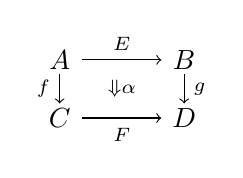
\begin{tikzpicture}[x=1.5em,y=1.5em]
  \node at (0,1.4) {$A$};
  \node at (3.0,1.4) {$B$};
  \draw[->] (0.55,1.4) -- node[above]{$\scriptstyle E$} (2.45,1.4);
  \draw[->] (0,1.05) -- node[left]{$\scriptstyle f$} (0,0.35);
  \draw[->] (3.0,1.05) -- node[right]{$\scriptstyle g$} (3.0,0.35);
  \node at (1.5,0.7) {$\scriptstyle\Downarrow\alpha$};
  \node at (0,0) {$C$};
  \node at (3.0,0) {$D$};
  \draw[->] (0.55,0) -- node[below]{$\scriptstyle F$} (2.45,0);
\end{tikzpicture}
\end{center}
\end{exercise}


